%File: main.tex
\documentclass[letterpaper]{article} % DO NOT CHANGE THIS
\usepackage{aaai24}  % DO NOT CHANGE THIS
\usepackage{times}  % DO NOT CHANGE THIS
\usepackage{helvet}  % DO NOT CHANGE THIS
\usepackage{courier}  % DO NOT CHANGE THIS
\renewcommand{\ttdefault}{lmtt}  % TinyTeX lacks Courier metrics; use Latin Modern Typewriter
\usepackage[hyphens]{url}  % DO NOT CHANGE THIS
\usepackage{graphicx} % DO NOT CHANGE THIS
\urlstyle{rm} % DO NOT CHANGE THIS
\def\UrlFont{\rm}  % DO NOT CHANGE THIS
\usepackage{natbib}  % DO NOT CHANGE THIS AND DO NOT ADD ANY OPTIONS TO IT
\usepackage{caption} % DO NOT CHANGE THIS AND DO NOT ADD ANY OPTIONS TO IT
\frenchspacing  % DO NOT CHANGE THIS
\setlength{\pdfpagewidth}{8.5in}  % DO NOT CHANGE THIS
\setlength{\pdfpageheight}{11in}  % DO NOT CHANGE THIS
\pdfinfo{
/TemplateVersion (2024.1)
}

\setcounter{secnumdepth}{1}

\title{Understanding the Effects of Learning Rate, Learning Rate Schedule, Weight Decay, and Mixup on EfficientNetV2-S Trained From Scratch}
\author{
    Jingtao Luo\textsuperscript{\rm 1}
}
\affiliations{
    \textsuperscript{\rm 1}Nanyang Technological University\\
    jingtao003@e.ntu.edu.sg
}

\begin{document}

\maketitle

\begin{abstract}
This report investigates the effects of learning rate, 
learning rate scheduling, weight decay, and data mixup on EfficientNetV2-S 
trained from scratch on the Dog Breed Identification dataset.
We first compare three initial learning rates, 
then evaluate constant and cosine-annealed learning rates, 
two weight decay coefficients, and data mixup
over 300 epochs. All experiments use SGD with momentum 0.9 and 
a consistent preprocessing pipeline. Training and validation 
losses and accuracies are reported for each configuration. 
The final mixup experiment achieves 32.7\% validation accuracy, 
and the checkpoint selected using validation accuracy achieves 33.38\%
accuracy on the hold-out test set.
\end{abstract}
\section{Introduction}

Deep neural networks are governed by two competing forces: optimization, which
controls how fast and how far training drives the loss down, and
regularization, which prevents the model from memorizing the training set.
The initial learning rate and its schedule control optimization, while weight
decay and data augmentation control regularization.  In this work we study
these four factors in a controlled manner on the Dog Breed Identification
dataset (10{,}222 images over 120 breeds; 7{,}155 training, 1{,}533
validation, and 1{,}534 test images), using EfficientNetV2-S from torchvision
\cite{tan2021efficientnetv2} trained from scratch with random initialization.
All experiments use SGD with momentum 0.9, batch size 128, and images resized
to $100\times100$; Table \ref{tab:setup} summarizes the fixed settings.
Training uses 12-pixel zero padding followed by a random
$100\times100$ crop and horizontal flipping with probability 0.5.
Hyperparameters are tuned on the validation set only; the test set is used
once, after all experiments are finished.  For every experiment we plot
training and validation loss and accuracy against the number of epochs, and
report the final training and validation losses and accuracies.

\begin{table}[tb]
\centering
\small
\begin{tabular}{ll}
\hline
model & EfficientNetV2-S (torchvision, random init) \\
optimizer & SGD (momentum$=0.9$) \\
batch size & 128 \\
image size & $100\times100$ \\
augmentation & zero pad + random crop + horizontal flip \\
normalization & per-channel z-score standardization \\
tuning & val only; test once at the end \\
\hline
\end{tabular}
\caption{Fixed settings shared by all experiments.}
\label{tab:setup}
\end{table}

\section{Data Preprocessing}

Before training we develop a sense of the data: the dataset contains 10{,}222
images split into 7{,}155 training, 1{,}533 validation, and 1{,}534 test
images across 120 dog breeds.  Every image is resized to $100\times100$.  Then
we apply per-channel z-score standardization, transforming each pixel channel
as
\[
z_c = \frac{x_c - \mu_c}{\sigma_c},
\]
where $z_c$ is the standardized pixel value, $x_c$ is the original pixel
value, and $\mu_c$ and $\sigma_c$ are the mean and standard deviation of
channel $c$ estimated on the training set only, giving
$\mu=[0.4772,0.4528,0.3928]$ and $\sigma=[0.2534,0.2480,0.2523]$.  The
validation and test splits use exactly the same normalization statistics
estimated from the training set, so no statistics are computed on the
validation or test data.  Note that this is channel-wise standardization
rather than full whitening, since channels are not decorrelated.
The training split additionally receives the required augmentation: 12 pixels
of zero padding on all four sides, a random $100\times100$ crop (equivalent to
a random translation of at most 12 pixels), and a horizontal flip with
probability 0.5.  The validation and test splits are not augmented.  Figure
\ref{lst:aug} shows the preprocessing code.

\begin{figure}[tb]
\centering
\begin{minipage}{0.92\columnwidth}
\scriptsize\ttfamily
\begin{verbatim}
steps = [Resize((100, 100), antialias=True)]
if split == "train":
    steps += [
        Pad(12, fill=0),
        RandomCrop(100),
        RandomHorizontalFlip(0.5),
    ]
steps += [ToTensor(), Normalize(mean, std)]
return Compose(steps)
\end{verbatim}
\end{minipage}
\caption{Per-split preprocessing pipeline (training split shown with the
required zero padding, random crop, and horizontal flip).}
\label{lst:aug}
\end{figure}

\section{Learning Rate}

We run three 15-epoch experiments with initial learning rates 0.5, 0.05, and
0.001, using neither weight decay nor a learning rate schedule, so that the
learning rate is the only varying factor.  Table \ref{tab:lr} reports the
final (epoch 15) losses and accuracies, and Figure \ref{fig:lr} shows the
training curves of the three runs.

\begin{table}[tb]
\centering
\small
\begin{tabular}{lcccc}
\hline
lr & train loss & train acc & val loss & val acc \\
\hline
0.5   & 4.7221 & 1.69\% & 4.7166 & 2.41\% \\
0.05  & 4.4190 & 3.63\% & 4.4719 & 3.46\% \\
0.001 & 4.8405 & 1.38\% & 5.0146 & 1.44\% \\
\hline
\end{tabular}
\caption{Final losses and accuracies of the three learning-rate experiments
after 15 epochs.}
\label{tab:lr}
\end{table}

\begin{figure}[tb]
\centering
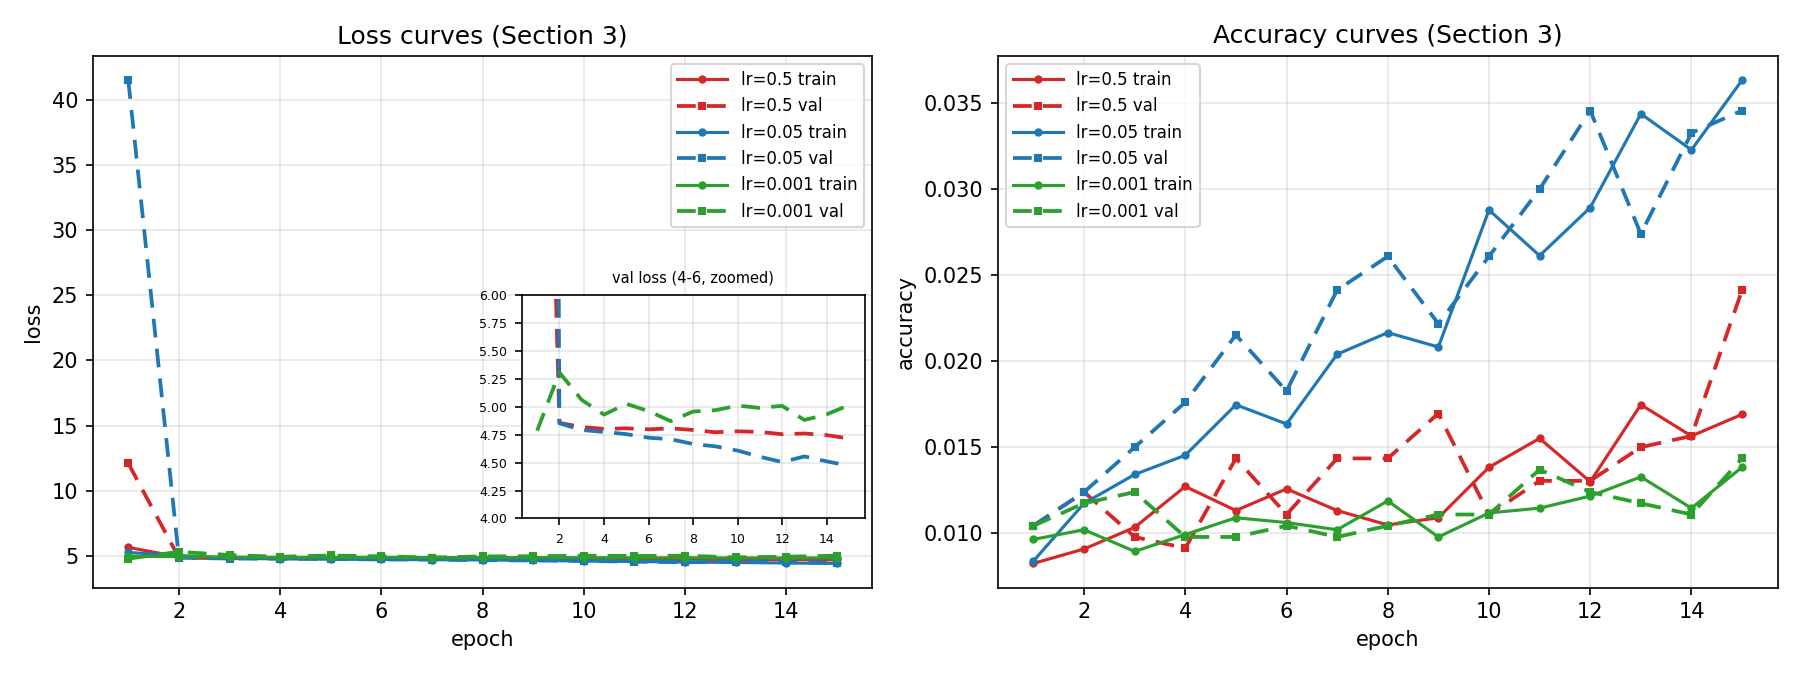
\includegraphics[width=\columnwidth]{figures/lr_comparison.png}
\caption{Loss and accuracy curves for learning rates 0.5, 0.05, and 0.001.}
\label{fig:lr}
\end{figure}

The best learning rate in terms of training loss is $0.05$, with a final
training loss of 4.4190; it also achieves the best validation loss (4.4719),
training accuracy (3.63\%), and validation accuracy (3.46\%) among the three.
The largest learning rate, 0.5, descends fastest in the first epochs, but its
large steps oscillate and settle at a higher loss.  The smallest learning
rate, 0.001, moves too slowly and its validation loss even rises to 5.01.
The three runs are far from convergence after 15 epochs (accuracies around
1--3.5\%, versus 0.8\% random chance), which motivates the longer runs below.
The initial validation-loss spikes (41.5 for lr 0.05, 12.1 for lr 0.5 in
epoch 1) reflect extreme logits of the randomly initialized network and vanish
quickly.  In summary, lr 0.05 gives the lowest training loss (4.4190) and
also the lowest validation loss (4.4719), the highest training accuracy
(3.63\%), and the highest validation accuracy (3.46\%) among the three; we
therefore fix the initial learning rate to 0.05 for the remaining
experiments.  At this stage the differences are dominated by optimization
speed rather than overfitting.

\section{Learning Rate Schedule}

Cosine annealing smoothly decreases the learning rate from an initial value
$\eta_{\max}$ to a minimum $\eta_{\min}$ over $T_{\max}$ epochs:
\begin{equation}
\eta_t = \eta_{\min} + \frac{\eta_{\max}-\eta_{\min}}{2}
\left(1 + \cos\left(\frac{\pi t}{T_{\max}}\right)\right).
\end{equation}
Intuitively, the schedule keeps large steps early to explore quickly and
shrinks the steps to zero so that the final phase fine-tunes the solution
without the oscillations a constant large step causes near the bottom of the
loss surface.  In our experiments $\eta_{\max}=0.05$, $\eta_{\min}=0$, and
$T_{\max}=300$, so $\eta_t=0.025(1+\cos(\pi t/300))$, implemented with
PyTorch's \texttt{CosineAnnealingLR}.

We compare two 300-epoch runs with the best learning rate 0.05 kept constant
versus annealed to zero by cosine annealing, with all other settings
unchanged.  Table \ref{tab:sched} reports the final metrics and Figure
\ref{fig:sched} the curves.

\begin{table}[tb]
\centering
\small
\begin{tabular}{lcccc}
\hline
condition & train loss & train acc & val loss & val acc \\
\hline
constant 0.05 & 0.0199 & 99.4\% & 9.8189 & 12.8\% \\
cosine annealing & 0.0039 & 99.9\% & 8.6630 & 17.2\% \\
\hline
\end{tabular}
\caption{Final metrics of the 300-epoch schedule experiments.}
\label{tab:sched}
\end{table}

\begin{figure}[tb]
\centering
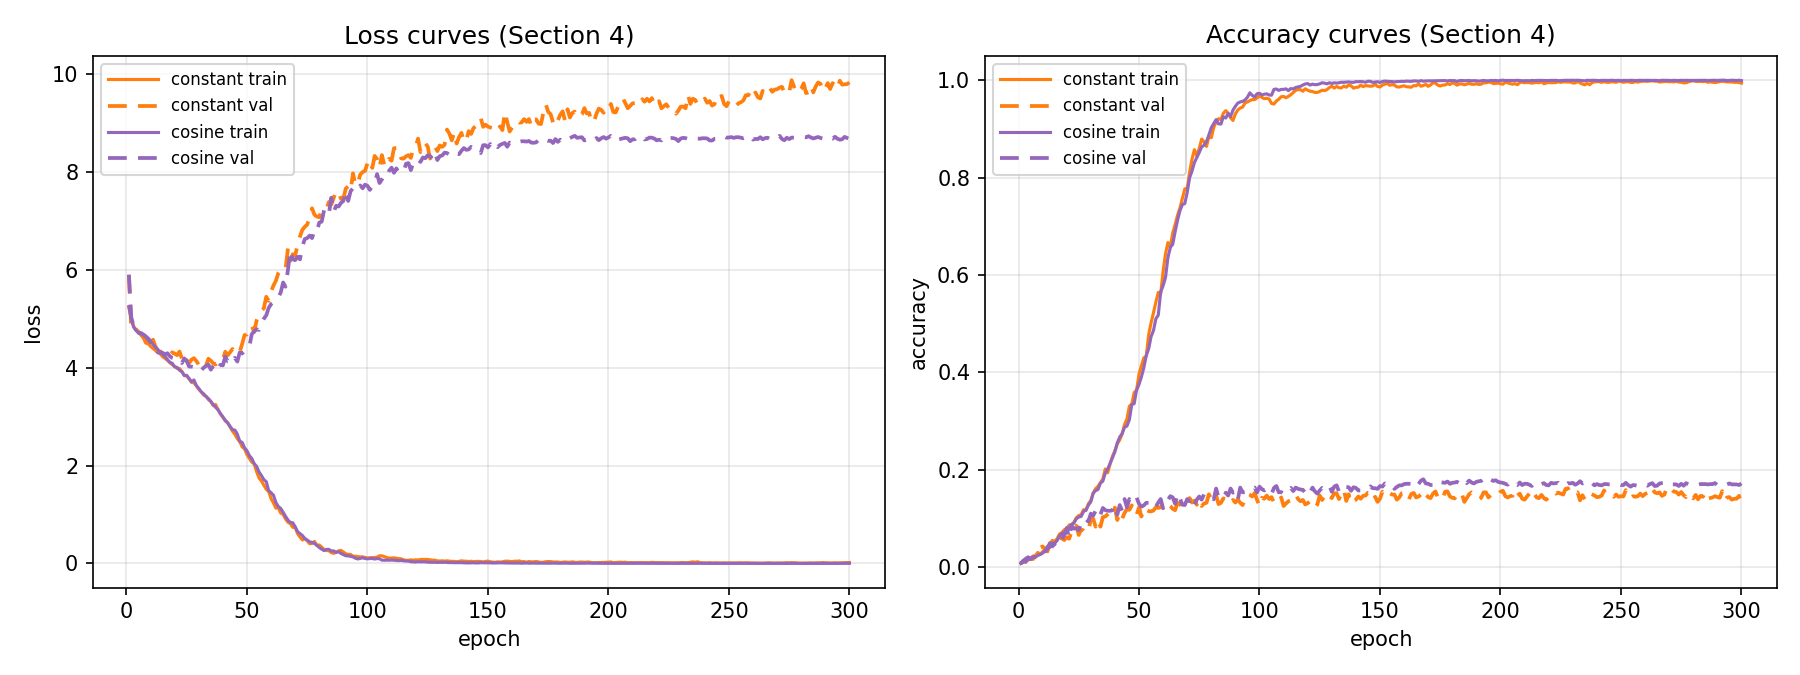
\includegraphics[width=\columnwidth]{figures/schedule_curves.png}
\caption{Constant versus cosine-annealed learning rate over 300 epochs.}
\label{fig:sched}
\end{figure}

\begin{figure}[tb]
\centering
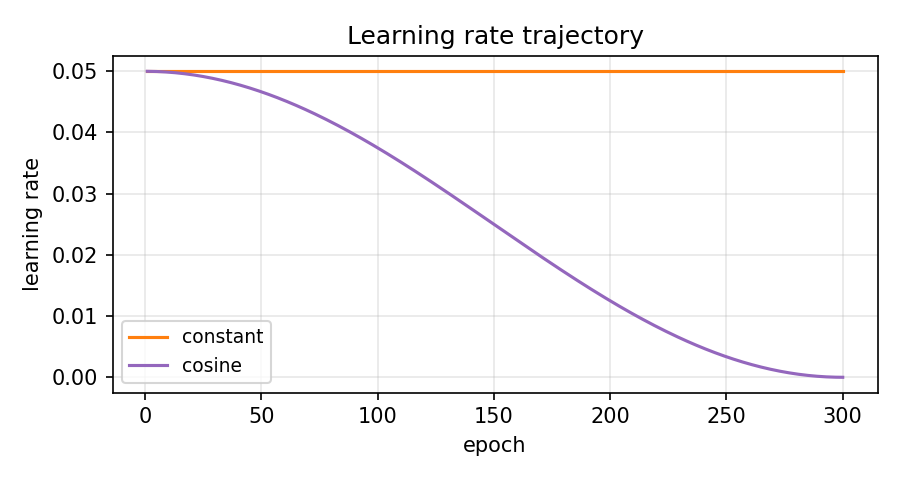
\includegraphics[width=\columnwidth]{figures/schedule_lr.png}
\caption{Learning-rate trajectory of the two schedule conditions.}
\label{fig:schedlr}
\end{figure}

Both conditions fit the training set almost perfectly, but their validation
trajectories differ sharply.  With a constant learning rate the validation
loss rises almost monotonically after epoch 50, from 4.68 to 9.82, and the
validation accuracy degrades late in training (best 16.3\% at epoch 269, final
12.8\%).  With cosine annealing the validation loss still rises (from 4.40 at
epoch 50) but stabilizes around 8.7 after epoch 200, ending at 8.66 with
17.2\% validation accuracy and a best value of 18.2\% at epoch 193.  A
constant step of size 0.05 keeps injecting gradient noise near the minimum,
so the weights wander and accumulate generalization error; annealing reduces
the step size and lets the optimizer settle, which simultaneously stabilizes
validation performance.  In summary, cosine annealing lowers the final
validation loss from 9.82 to 8.66 and raises the final validation accuracy
from 12.8\% to 17.2\%, so we adopt the cosine schedule for all subsequent
runs.

\section{Weight Decay}

Adding a quadratic penalty to an arbitrary loss $L(w)$ gives
\begin{equation}
L'(w) = L(w) + \frac{\lambda}{2}\|w\|^2 
\end{equation}
Here $\lambda$ is the weight decay coefficient that controls the strength of the
penalty. Differentiating and writing the gradient descent update for
$L'(w)$ gives
\begin{eqnarray*}
w_{t+1} &= w_t - \eta\,\frac{\partial L(w_t)}{\partial w_t}
- \eta\lambda w_t \\
&= \left(1 - \eta\lambda\right) w_t
- \eta\,\frac{\partial L(w_t)}{\partial w_t} 
\end{eqnarray*}
The factor $(1-\eta\lambda)$ shows that each update first shrinks
every weight by a fixed fraction $\eta\lambda$ before applying the gradient
step.  Instead of optimizing $L'(w)$ directly, one can therefore run plain
gradient descent on $L(w)$ and subtract $\eta\lambda $ from the weights in
each update. In our experiments, we use PyTorch's SGD optimizer with 
momentum 0.9 and the built-in \texttt{weight\_decay} parameter,
which incorporates the L2 penalty into the gradient before the momentum update
\cite{zhang2019three}.
We keep the best configuration so far (initial learning rate 0.05 plus cosine
annealing) and train 300 epochs with $\lambda=5\times10^{-4}$ and
$\lambda=1\times10^{-4}$.  Table \ref{tab:wd} and Figure \ref{fig:wd} compare
the two runs against the no-decay cosine baseline.

\begin{table}[tb]
\centering
\small
\begin{tabular}{lcccc}
\hline
condition & train loss & train acc & val loss & val acc \\
\hline
no decay & 0.0039 & 99.9\% & 8.6630 & 17.2\% \\
$\lambda=5\times10^{-4}$ & 0.0198 & 99.9\% & 3.7447 & 27.7\% \\
$\lambda=1\times10^{-4}$ & 0.0056 & 99.9\% & 6.9302 & 16.8\% \\
\hline
\end{tabular}
\caption{Final metrics of the weight decay experiments (300 epochs).}
\label{tab:wd}
\end{table}

\begin{figure}[tb]
\centering
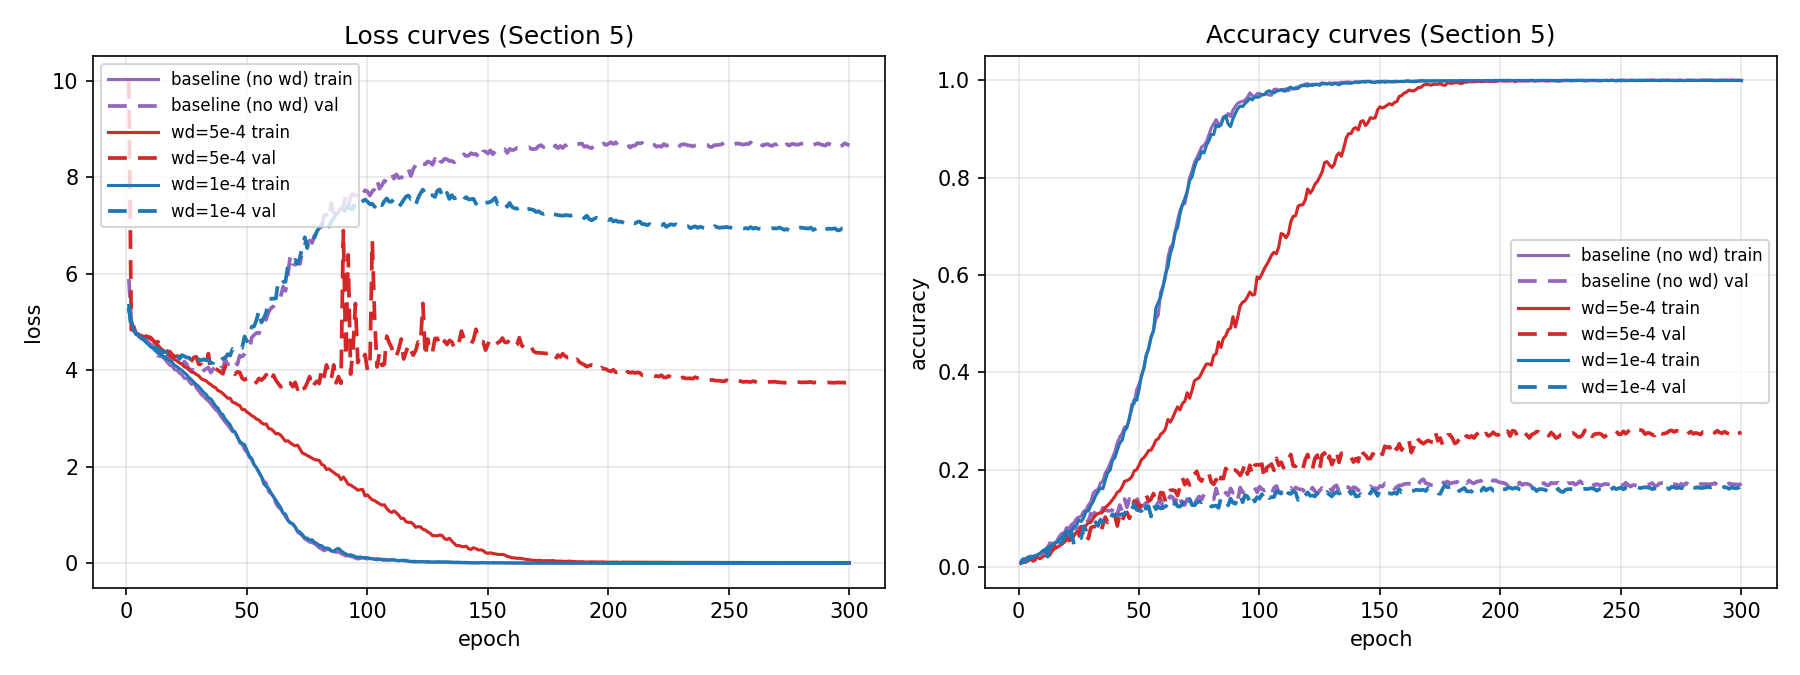
\includegraphics[width=\columnwidth]{figures/wd_comparison.png}
\caption{Weight decay 5e-4 and 1e-4 versus the no-decay cosine baseline.}
\label{fig:wd}
\end{figure}

Weight decay with $\lambda=5\times10^{-4}$ is the single most effective change
so far: final validation loss drops from 8.66 to 3.74 and validation accuracy
rises from 17.2\% to 27.7\% (best 28.3\% at epoch 254), while the training set
is still fitted (99.9\%).  The weak decay $\lambda=1\times10^{-4}$ behaves
almost like the baseline: its decay term is too small relative to the
gradient updates to restrain the weight norm, so memorization proceeds as
before.  A notable phenomenon is that the 5e-4 validation
loss first rises (3.83 at epoch 50 to 4.55 at epoch 150) and then falls to
3.74: early on the model still overfits somewhat, but as cosine annealing
shrinks the learning rate and the decay term keeps contracting the weights,
the solution moves back toward smoother regions and generalization improves.
This directly illustrates the regularizing role of weight decay: by shrinking
the weight norm each step it constrains the effective hypothesis space and
slows down the memorization of training noise.  In summary, the stronger
decay $\lambda=5\times10^{-4}$ cuts the final validation loss from 8.66 to
3.74 and raises the validation accuracy from 17.2\% to 27.7\%, and we adopt
it for the remaining experiment.

\section{Data Augmentation: Mixup}

Mixup trains on convex combinations of input pairs with the same interpolation
applied to the labels gives
\begin{equation}
\tilde{x} = \lambda x_i + (1-\lambda) x_j
\tilde{y} = \lambda y_i + (1-\lambda) y_j
\end{equation}
where $\lambda$ follows a Beta distribution
\cite{zhang2018mixup}. 

\begin{figure}[tb]
\centering
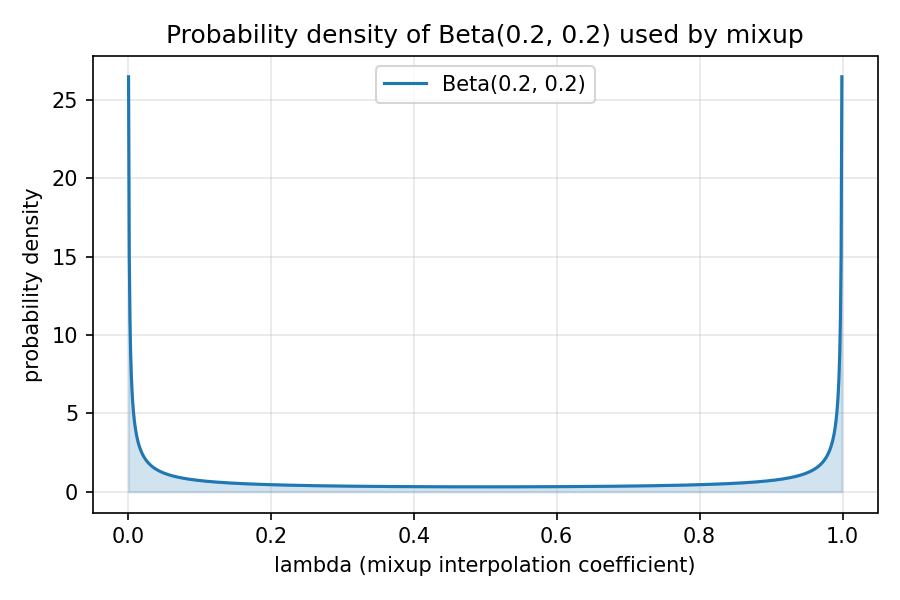
\includegraphics[width=0.62\columnwidth]{figures/beta_pdf.png}
\caption{Probability density of $\mathrm{Beta}(0.2,0.2)$, the distribution of
the mixup interpolation coefficient.}
\label{fig:beta}
\end{figure}

The shape parameter $\alpha$ controls this mixing distribution: small
$\alpha$ concentrates the density near $\lambda=0$ and $\lambda=1$, so most
updates interpolate only mildly, while large $\alpha$ pushes the mass toward
$\lambda=0.5$, i.e., stronger blending of the two images and labels.
With $\alpha=0.2$ the density puts most mass near
$\lambda=0$ and $\lambda=1$ (mild mixing), with occasional near-50/50 blends,
as shown in Figure \ref{fig:beta}.

We apply mixup with $\alpha=0.2$ to the best configuration so far (learning
rate 0.05, cosine annealing, weight decay $5\times10^{-4}$) and train for 300
epochs.  Table \ref{tab:mixup} and Figure \ref{fig:mixup} compare against the
same configuration without mixup.

\begin{table}[tb]
\centering
\small
\begin{tabular}{lcccc}
\hline
condition & train loss & train acc & val loss & val acc \\
\hline
no mixup & 0.0198 & 99.9\% & 3.7447 & 27.7\% \\
mixup $\alpha=0.2$ & 0.7844 & 89.5\% & 3.0175 & 32.7\% \\
\hline
\end{tabular}
\caption{Final metrics with and without mixup (300 epochs).}
\label{tab:mixup}
\end{table}

\begin{figure}[tb]
\centering
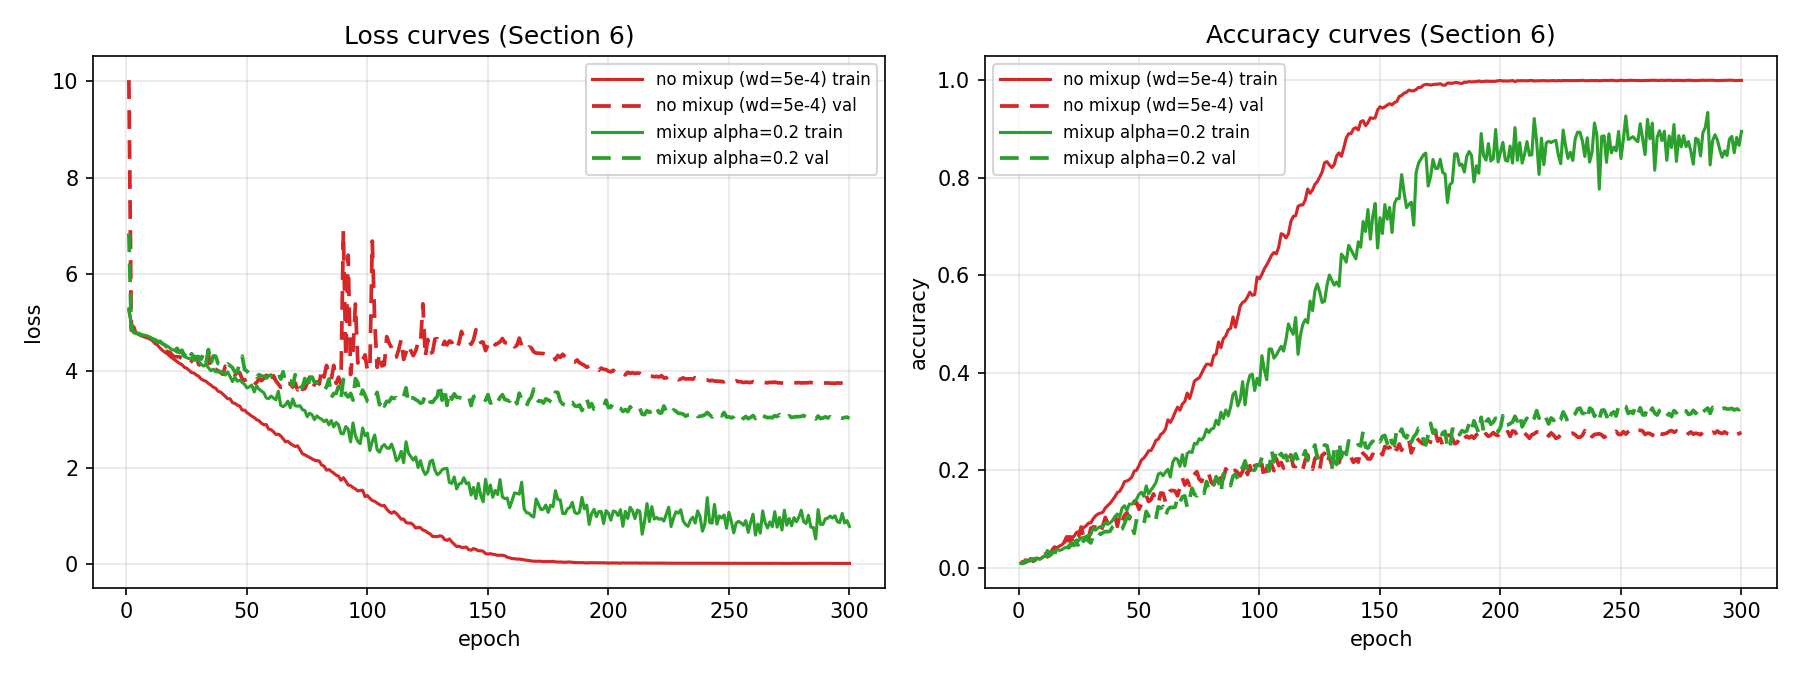
\includegraphics[width=\columnwidth]{figures/mixup_comparison.png}
\caption{Mixup $\alpha=0.2$ versus the identical configuration without mixup.}
\label{fig:mixup}
\end{figure}

With mixup, the finaltraining accuracy stays 
at 89.5\% (versus 99.9\% without mixup).  Note that the reported training
accuracy with mixup is the $\lambda$-weighted soft accuracy evaluated on the
mixed images and mixed labels, i.e.,
$\lambda\,\mathbf{1}[f(\tilde{x})=y_i]
+(1-\lambda)\,\mathbf{1}[f(\tilde{x})=y_j]$ averaged over the batch; it is
not the hard accuracy on the original unmodified training images.  The
validation accuracy, in contrast, is always measured on the original
(unmixed) validation images, so the two accuracies are not directly
comparable.  At the same time the validation loss improves from 3.74 to 3.02
and validation accuracy from 27.7\% to 32.7\% (best 33.2\% at epoch 251).
The validation loss decreases almost monotonically after epoch 100.  
Mixup acts as data-level regularization: it reduces over-confidence 
on individual examples.

Finally, we evaluate the checkpoint selected by the validation protocol
(epoch 251, the highest validation accuracy, 33.2\%) once on the hold-out
test set of 1{,}534 images: the test loss is 3.000 and the test accuracy is
\textbf{33.38\%}. Mixup and weight decay thus act on different
levels---the data distribution and the parameter space---and their
combination gives the best generalization of all configurations. We select
the best checkpoint rather than the final one because choosing the model by
validation performance is part of the validation-only tuning protocol; the
two choices differ little here (best 33.2\% versus final 32.7\% validation
accuracy), and the best checkpoint slightly favors generalization.  In
summary, mixup raises the validation accuracy from 27.7\% to 32.7\% and the 
selected model reaches 33.38\% on the hold-out test set.

\section{Take Away Message}

No conclusion due to the rubric of this assignment\cite{li2026ai6103}. 
You will find out if you read the report carefully.

\begin{thebibliography}{}

\bibitem[Tan and Le, 2021]{tan2021efficientnetv2}
Tan, M.; and Le, Q. V. 2021.
EfficientNetV2: Smaller Models and Faster Training.
In \emph{Proceedings of the 38th International Conference on Machine
Learning}, 10096--10106.

\bibitem[Loshchilov and Hutter, 2017]{loshchilov2017sgdr}
Loshchilov, I.; and Hutter, F. 2017.
SGDR: Stochastic Gradient Descent with Warm Restarts.
In \emph{Proceedings of the 5th International Conference on Learning
Representations}.

\bibitem[Zhang et al., 2019]{zhang2019three}
Zhang, G.; Wang, C.; Xu, B.; and Grosse, R. 2019.
Three Mechanisms of Weight Decay Regularization.
In \emph{Proceedings of the 7th International Conference on Learning
Representations}.

\bibitem[Zhang et al., 2018]{zhang2018mixup}
Zhang, H.; Cisse, M.; Dauphin, Y. N.; and Lopez-Paz, D. 2018.
mixup: Beyond Empirical Risk Minimization.
In \emph{Proceedings of the 6th International Conference on Learning
Representations}.

\bibitem[PyTorch, 2024]{torchvision}
PyTorch. 2024. torchvision: EfficientNetV2-S.
\url{https://pytorch.org/vision/stable/models/efficientnetv2.html}.

\bibitem[Li, 2026]{li2026ai6103}
Li, B. 2026.
AI6103 Homework Assignment.
Unpublished course assignment handout,
Nanyang Technological University.

\end{thebibliography}

\end{document}
